\part{Appendix}%
\label{ch:appendix}

\chapter{Running Example in the Palladio Component Model}%
\label{sec:appendix:runningexample}

Our running example is shown in \autoref{ch:runningexample}.
To illustrate the architectural model of the running example using the \acf{PCM}, we show two diagrams.
First, \autoref{fig:appendix:runningexample:repository} shows a graphical representation of the Palladio \emph{component repository model}, comprising the components and their interfaces.
Second, \autoref{fig:appendix:runningexample:seff} shows the \acf{SEFF} of \emph{purchaseItem}, comprising the default purchasing behavior and alternatives due to uncertainty, e.g., the processing of purchase data with erroneous encryption, or lacking validation.
The behavior is represented using assignments, e.g., by assigning the \emph{Validated} and \emph{Encrypted} labels in the upper left, as defined by \textcite{seifermann_identifying_2021}.

Both diagrams are exported from the Palladio Bench \cite{reussner_palladio_2024}, which represents the foundation of our tool support.
The diagrams can be created and altered using Eclipse's inline diagram editors.
Furthermore, \autoref{fig:appendix:runningexample:uncertainty} shows an excerpt from our tool support to create uncertainty models, following the meta model presented in \autoref{fig:confidentialityanalysis:uncertaintymetamodelpcm}.
Here, the uncertainty scenarios of the \emph{Behavior} uncertainty \U{2} reference the alternative actions shown in \autoref{fig:appendix:runningexample:seff}.
Using these models and previously specified data flow constraints \cite{hahner_modeling_2021,boltz_extensible_2024} as an input, \abunai can identify confidentiality violations due to uncertainty, see \autoref{sec:confidentialityanalysis:abunai}.
The remaining \ac{PCM} models and the required tooling to display them can be found in the data set \cite{dataset}.

\begin{figure}
    \centering
    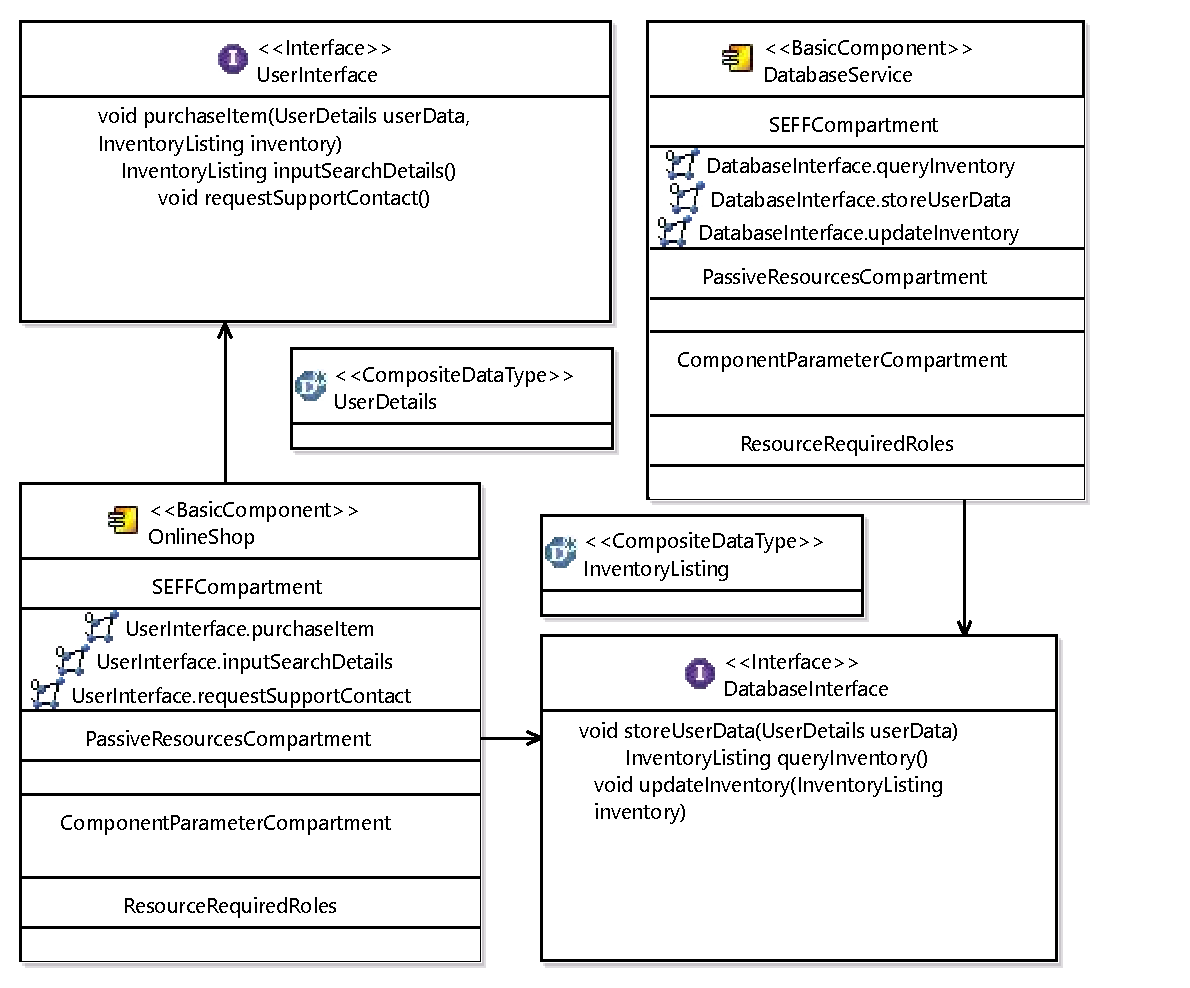
\includegraphics[width=\textwidth]{figures/chapter12/runningexample_repository.pdf}
    \caption[Palladio repository model of the running example.]{Palladio repository model of the running example, exported from the Palladio-Bench \cite{reussner_palladio_2024}.}
    \label{fig:appendix:runningexample:repository}
\end{figure}

\begin{figure}
    \centering
    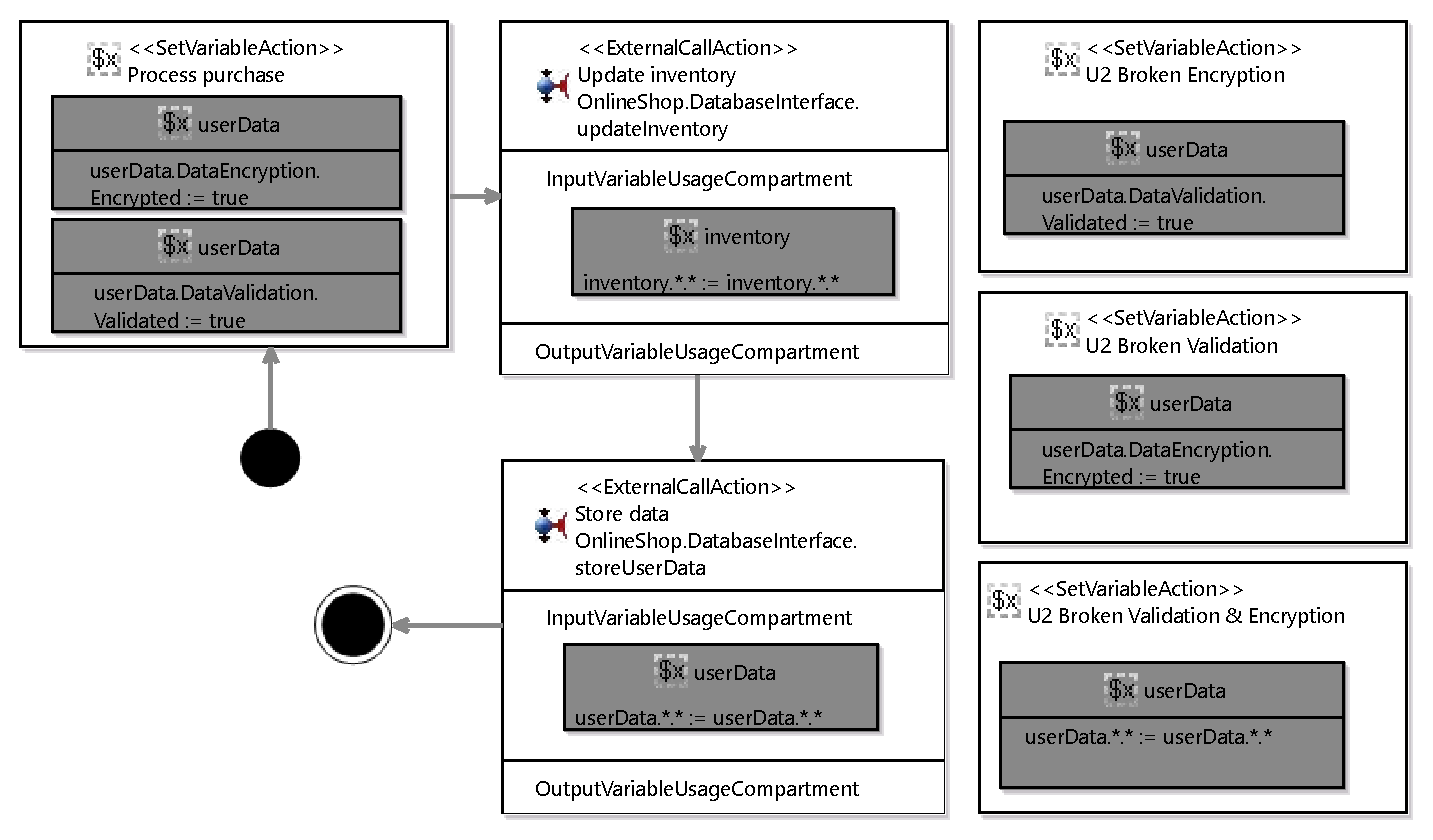
\includegraphics[width=\textwidth]{figures/chapter12/runningexample_seff.pdf}
    \caption[Exemplary Palladio \acf*{SEFF} of the running example.]{Exemplary Palladio \acf*{SEFF} of the running example, exported from the Palladio-Bench \cite{reussner_palladio_2024}.}
    \label{fig:appendix:runningexample:seff}
\end{figure}

\begin{figure}
    \centering
    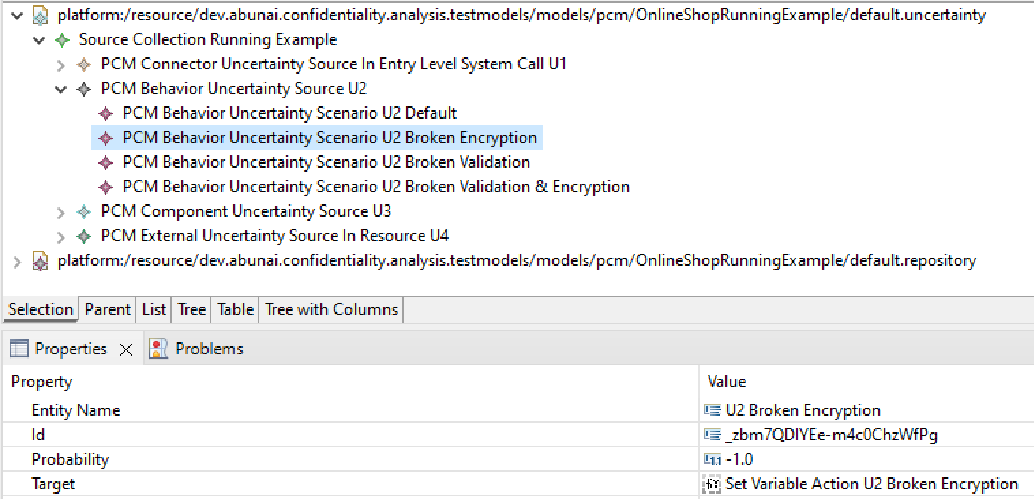
\includegraphics[width=\textwidth]{figures/chapter12/runningexample_uncertainty.pdf}
    \caption[Uncertainty model of the running example, showing four uncertainty sources and their scenarios.]{Uncertainty model of the running example, showing four uncertainty sources and their scenarios. Screenshot from the Palladio-Bench \cite{reussner_palladio_2024}.}
    \label{fig:appendix:runningexample:uncertainty}
\end{figure}





\chapter{Impact Sets of the Running Example}%
\label{sec:appendix:impactset}

Our uncertainty impact analysis has been introduced in \autoref{ch:impactanalysis}.
We show the resulting impact sets after the architectural propagation and the propagation in the \acf{DFD} of the running example, see \autoref{ch:runningexample}.
These are the results of the automated uncertainty impact analysis \uia.
\autoref{lst:appendix:impactset:u1} shows the impact set of Uncertainty \U{1}, \autoref{lst:appendix:impactset:u2} shows the impact set of Uncertainty \U{2}, \autoref{lst:appendix:impactset:u3} shows the impact set of Uncertainty \U{3}, and \autoref{lst:appendix:impactset:u4} shows the impact set of Uncertainty \U{4}.
We removed the element IDs from the analysis output for the sake of brevity.
The comprehensive analysis output can be found in the data set \cite{dataset}.

\begin{figure}
    \begin{lstlisting}[
        style=appendix,
        caption={Result of the uncertainty impact analysis of Uncertainty \U{1} in the running example.},
        label={lst:appendix:impactset:u1}
    ]
    Result of the PCM propagation:
    SEFFActionSequenceElement (Beginning view)
    SEFFActionSequenceElement (Beginning buy)
    SEFFActionSequenceElement (Beginning requestSupport)
    SEFFActionSequenceElement (Beginning view)
    CallingUserActionSequenceElement / calling (ViewEntryLevelSystemCall)
    CallingUserActionSequenceElement / returning (ViewEntryLevelSystemCall)
    CallingUserActionSequenceElement / calling (BuyEntryLevelSystemCall)
    CallingUserActionSequenceElement / returning (BuyEntryLevelSystemCall)
    CallingUserActionSequenceElement / calling (RequestSupportCall)
    CallingUserActionSequenceElement / returning (RequestSupportCall)
    CallingUserActionSequenceElement / calling (ViewShopCall)
    CallingUserActionSequenceElement / returning (ViewShopCall)
    Result of the DFD propagation:
    CallingUserActionSequenceElement / calling (ViewShopCall)
    SEFFActionSequenceElement (Beginning view)
    CallingSEFFActionSequenceElement / calling (DatabaseLoadInventory)
    SEFFActionSequenceElement (Beginning loadInventory)
    SEFFActionSequenceElement (RETURN)
    SEFFActionSequenceElement (Ending loadInventory)
    CallingSEFFActionSequenceElement / returning (DatabaseLoadInventory)
    SEFFActionSequenceElement (RETURN)
    SEFFActionSequenceElement (Ending view)
    CallingUserActionSequenceElement / returning (ViewShopCall)
    UserActionSequenceElement (Stopping usage: View Shop)
    CallingUserActionSequenceElement / calling (ViewEntryLevelSystemCall)
    SEFFActionSequenceElement (Beginning view)
    CallingSEFFActionSequenceElement / calling (DatabaseLoadInventory)
    SEFFActionSequenceElement (Beginning loadInventory)
    SEFFActionSequenceElement (RETURN)
    SEFFActionSequenceElement (Ending loadInventory)
    CallingSEFFActionSequenceElement / returning (DatabaseLoadInventory)
    SEFFActionSequenceElement (RETURN)
    SEFFActionSequenceElement (Ending view)
    CallingUserActionSequenceElement / returning (ViewEntryLevelSystemCall)
    CallingUserActionSequenceElement / calling (BuyEntryLevelSystemCall)
    SEFFActionSequenceElement (Beginning buy)
    SEFFActionSequenceElement (UserDataProcessing)
    CallingSEFFActionSequenceElement / calling (DatabaseStoreInventory)
    SEFFActionSequenceElement (Beginning updateInventory)
    SEFFActionSequenceElement (Ending updateInventory)
    CallingSEFFActionSequenceElement / returning (DatabaseStoreInventory)
    CallingSEFFActionSequenceElement / calling (DatabaseStoreUserData)
    SEFFActionSequenceElement (Beginning storeUserData)
    SEFFActionSequenceElement (Ending storeUserData)
    CallingSEFFActionSequenceElement / returning (DatabaseStoreUserData)
    SEFFActionSequenceElement (Ending buy)
    CallingUserActionSequenceElement / returning (BuyEntryLevelSystemCall)
    UserActionSequenceElement (Stopping usage: Buy from Shop)
    CallingUserActionSequenceElement / calling (RequestSupportCall)
    SEFFActionSequenceElement (Beginning requestSupport)
    SEFFActionSequenceElement (Ending requestSupport)
    CallingUserActionSequenceElement / returning (RequestSupportCall)
    UserActionSequenceElement (Stopping usage: Request Support)
    \end{lstlisting}
\end{figure}

\begin{figure}
    \begin{lstlisting}[
        style=appendix,
        caption={Result of the uncertainty impact analysis of Uncertainty \U{2} in the running example.},
        label={lst:appendix:impactset:u2}
    ]
    Result of the PCM propagation:
    SEFFActionSequenceElement (UserDataProcessing)

    Result of the DFD propagation:
    SEFFActionSequenceElement (UserDataProcessing)
    CallingSEFFActionSequenceElement / calling (DatabaseStoreInventory)
    SEFFActionSequenceElement (Beginning updateInventory)
    SEFFActionSequenceElement (Ending updateInventory)
    CallingSEFFActionSequenceElement / returning (DatabaseStoreInventory)
    CallingSEFFActionSequenceElement / calling (DatabaseStoreUserData)
    SEFFActionSequenceElement (Beginning storeUserData)
    SEFFActionSequenceElement (Ending storeUserData)
    CallingSEFFActionSequenceElement / returning (DatabaseStoreUserData)
    SEFFActionSequenceElement (Ending buy)
    CallingUserActionSequenceElement / returning (BuyEntryLevelSystemCall)
    UserActionSequenceElement (Stopping usage: Buy from Shop)
    \end{lstlisting}
\end{figure}

\begin{figure}
    \begin{lstlisting}[
        style=appendix,
        caption={Result of the uncertainty impact analysis of Uncertainty \U{3} in the running example.},
        label={lst:appendix:impactset:u3}
    ]
    Result of the PCM propagation:
    SEFFActionSequenceElement (Beginning loadInventory)
    SEFFActionSequenceElement (Beginning updateInventory)
    SEFFActionSequenceElement (Beginning storeUserData)
    SEFFActionSequenceElement (Beginning loadInventory)
    
    Result of the DFD propagation:
    SEFFActionSequenceElement (Beginning loadInventory)
    SEFFActionSequenceElement (RETURN)
    SEFFActionSequenceElement (Ending loadInventory)
    CallingSEFFActionSequenceElement / returning (DatabaseLoadInventory)
    SEFFActionSequenceElement (RETURN)
    SEFFActionSequenceElement (Ending view)
    CallingUserActionSequenceElement / returning (ViewShopCall)
    UserActionSequenceElement (Stopping usage: View Shop)
    SEFFActionSequenceElement (Beginning loadInventory)
    SEFFActionSequenceElement (RETURN)
    SEFFActionSequenceElement (Ending loadInventory)
    CallingSEFFActionSequenceElement / returning (DatabaseLoadInventory)
    SEFFActionSequenceElement (RETURN)
    SEFFActionSequenceElement (Ending view)
    CallingUserActionSequenceElement / returning (ViewEntryLevelSystemCall)
    CallingUserActionSequenceElement / calling (BuyEntryLevelSystemCall)
    SEFFActionSequenceElement (Beginning buy)
    SEFFActionSequenceElement (UserDataProcessing)
    CallingSEFFActionSequenceElement / calling (DatabaseStoreInventory)
    SEFFActionSequenceElement (Beginning updateInventory)
    SEFFActionSequenceElement (Ending updateInventory)
    CallingSEFFActionSequenceElement / returning (DatabaseStoreInventory)
    CallingSEFFActionSequenceElement / calling (DatabaseStoreUserData)
    SEFFActionSequenceElement (Beginning storeUserData)
    SEFFActionSequenceElement (Ending storeUserData)
    CallingSEFFActionSequenceElement / returning (DatabaseStoreUserData)
    SEFFActionSequenceElement (Ending buy)
    CallingUserActionSequenceElement / returning (BuyEntryLevelSystemCall)
    UserActionSequenceElement (Stopping usage: Buy from Shop)
    \end{lstlisting}
\end{figure}

\begin{figure}
    \begin{lstlisting}[
        style=appendix,
        caption={Result of the uncertainty impact analysis of Uncertainty \U{4} in the running example.},
        label={lst:appendix:impactset:u4}
    ]
    Result of the PCM propagation:
    SEFFActionSequenceElement (Beginning loadInventory)
    SEFFActionSequenceElement (RETURN)
    SEFFActionSequenceElement (Ending loadInventory)
    SEFFActionSequenceElement (Beginning updateInventory)
    SEFFActionSequenceElement (Ending updateInventory)
    SEFFActionSequenceElement (Beginning storeUserData)
    SEFFActionSequenceElement (Ending storeUserData)
    SEFFActionSequenceElement (Beginning loadInventory)
    SEFFActionSequenceElement (RETURN)
    SEFFActionSequenceElement (Ending loadInventory)

    Result of the DFD propagation:
    SEFFActionSequenceElement (Beginning loadInventory)
    SEFFActionSequenceElement (RETURN)
    SEFFActionSequenceElement (Ending loadInventory)
    CallingSEFFActionSequenceElement / returning (DatabaseLoadInventory)
    SEFFActionSequenceElement (RETURN)
    SEFFActionSequenceElement (Ending view)
    CallingUserActionSequenceElement / returning (ViewEntryLevelSystemCall)
    CallingUserActionSequenceElement / calling (BuyEntryLevelSystemCall)
    SEFFActionSequenceElement (Beginning buy)
    SEFFActionSequenceElement (UserDataProcessing)
    CallingSEFFActionSequenceElement / calling (DatabaseStoreInventory)
    SEFFActionSequenceElement (Beginning updateInventory)
    SEFFActionSequenceElement (Ending updateInventory)
    CallingSEFFActionSequenceElement / returning (DatabaseStoreInventory)
    CallingSEFFActionSequenceElement / calling (DatabaseStoreUserData)
    SEFFActionSequenceElement (Beginning storeUserData)
    SEFFActionSequenceElement (Ending storeUserData)
    CallingSEFFActionSequenceElement / returning (DatabaseStoreUserData)
    SEFFActionSequenceElement (Ending buy)
    CallingUserActionSequenceElement / returning (BuyEntryLevelSystemCall)
    UserActionSequenceElement (Stopping usage: Buy from Shop)
    SEFFActionSequenceElement (Beginning loadInventory)
    SEFFActionSequenceElement (RETURN)
    SEFFActionSequenceElement (Ending loadInventory)
    CallingSEFFActionSequenceElement / returning (DatabaseLoadInventory)
    SEFFActionSequenceElement (RETURN)
    SEFFActionSequenceElement (Ending view)
    CallingUserActionSequenceElement / returning (ViewShopCall)
    UserActionSequenceElement (Stopping usage: View Shop)
    \end{lstlisting}
\end{figure}





\chapter{All Confidentiality Violations in the Running Example}%
\label{sec:appendix:confidentiality}

We give an overview of all confidentiality violations identified in the running example by \abunai.
First, \autoref{lst:appendix:confidentiality:overview} shows all combinations of uncertainty scenarios that cause the violation of at least one confidentiality requirement.
Second, \autoref{lst:appendix:confidentiality:detail} exemplifies the result of the first scenario combination by showing all confidentiality-violating vertices.
The full analysis results can be found in the data set \cite{dataset}.

\begin{figure}
    \begin{lstlisting}[
        style=appendix,
        caption={All uncertainty scenarios of the running example that cause confidentiality violations.},
        label={lst:appendix:confidentiality:overview}
    ]
    [U1 Invalid, U2-Default, U3 Alternative]
    [U1 Invalid, U2 Broken Encryption, U3 Alternative]
    [U1 Invalid, U2 Broken Validation, U3 Alternative] 
    [U1 Invalid, U2 Broken Validation & Encryption, U3 Alternative]
    [U1 Invalid, U2-Default, U3-Default, U4-Default]
    [U1 Invalid, U2-Default, U3-Default, U4 Alternative]
    [U1 Invalid, U2 Broken Encryption, U3-Default, U4-Default]
    [U1 Invalid, U2 Broken Encryption, U3-Default, U4 Alternative]
    [U1 Invalid, U2 Broken Validation, U3-Default, U4-Default]
    [U1 Invalid, U2 Broken Validation, U3-Default, U4 Alternative]
    [U1 Invalid, U2 Broken Validation & Encryption, U3-Default, U4-Default]
    [U1 Invalid, U2 Broken Validation & Encryption, U3-Default, U4 Alternative]
    [U1-Default, U2 Broken Encryption, U3-Default, U4-Default]
    [U1-Default, U2 Broken Encryption, U3-Default, U4 Alternative]
    [U1-Default, U2 Broken Validation & Encryption, U3-Default, U4-Default]
    [U1-Default, U2 Broken Validation & Encryption, U3-Default, U4 Alternative]
    [U1 Invalid, U2 Broken Encryption, U3-Default, U4-Default]
    [U1 Invalid, U2 Broken Encryption, U3-Default, U4 Alternative]
    [U1 Invalid, U2 Broken Validation & Encryption, U3-Default, U4-Default]
    [U1 Invalid, U2 Broken Validation & Encryption, U3-Default, U4 Alternative]
    [U1 Malicious, U2 Broken Encryption, U3-Default, U4-Default]
    [U1 Malicious, U2 Broken Encryption, U3-Default, U4 Alternative]
    [U1 Malicious, U2 Broken Validation & Encryption, U3-Default, U4-Default]
    [U1 Malicious, U2 Broken Validation & Encryption, U3-Default, U4 Alternative]
    \end{lstlisting}
\end{figure}

\begin{figure}
    \begin{lstlisting}[
        style=appendix,
        caption={Detailed result of the first confidentiality violation of the running example.},
        label={lst:appendix:confidentiality:detail}
    ]
    [U1 Invalid, U2-Default, U3 Alternative] -> 
    {SEFFPCMVertex (Beginning purchaseItem,
    _nGp9cITjEeywmO_IpTxeAg), SEFFPCMVertex (Process purchase, _oEBNYDIXEe-m4c0ChzWfPg),
    CallingSEFFPCMVertex / calling (Update inventory, _yVL18ITkEeywmO_IpTxeAg), 
    CallingSEFFPCMVertex / returning (Update inventory, _yVL18ITkEeywmO_IpTxeAg),
    CallingSEFFPCMVertex / calling (Store data, _11NAEITkEeywmO_IpTxeAg), SEFFPCMVertex 
    (Beginning storeUserData, _oGmXgYTjEeywmO_IpTxeAg), SEFFPCMVertex (Ending 
    storeUserData, _oGmXgoTjEeywmO_IpTxeAg), CallingSEFFPCMVertex / returning (Store 
    data, _11NAEITkEeywmO_IpTxeAg), SEFFPCMVertex (Ending purchaseItem, 
    _nGp9cYTjEeywmO_IpTxeAg), CallingUserPCMVertex / returning (U1 Purchase item 
    Invalid, _UQNBoC1WEe-lUc5YrocPyg), UserPCMVertex (Stopping usage: Buy from Shop, 
    _LPwS4iHdEd6lJo4DCALHMw)},
    \end{lstlisting}
\end{figure}





\chapter{Palladio Repository Model of the Corona Warn App}%
\label{sec:appendix:cwa}

In the following, we show the full Palladio \emph{component repository model} of the \emph{Corona Warn App} evaluation scenario, see \autoref{sec:evaluationscenarios:coronawarnapp}.
Due to the large size of this diagram, we split it into four parts, shown in \autoref{fig:appendix:cwa:1}, \autoref{fig:appendix:cwa:2}, \autoref{fig:appendix:cwa:3}, and \autoref{fig:appendix:cwa:4}.
\autoref{fig:appendix:cwa:overview} gives an overview of the structure.
The original full-sized diagram and all \ac{PCM} model files can be found in the data set \cite{dataset}.

\begin{figure}
    \centering
    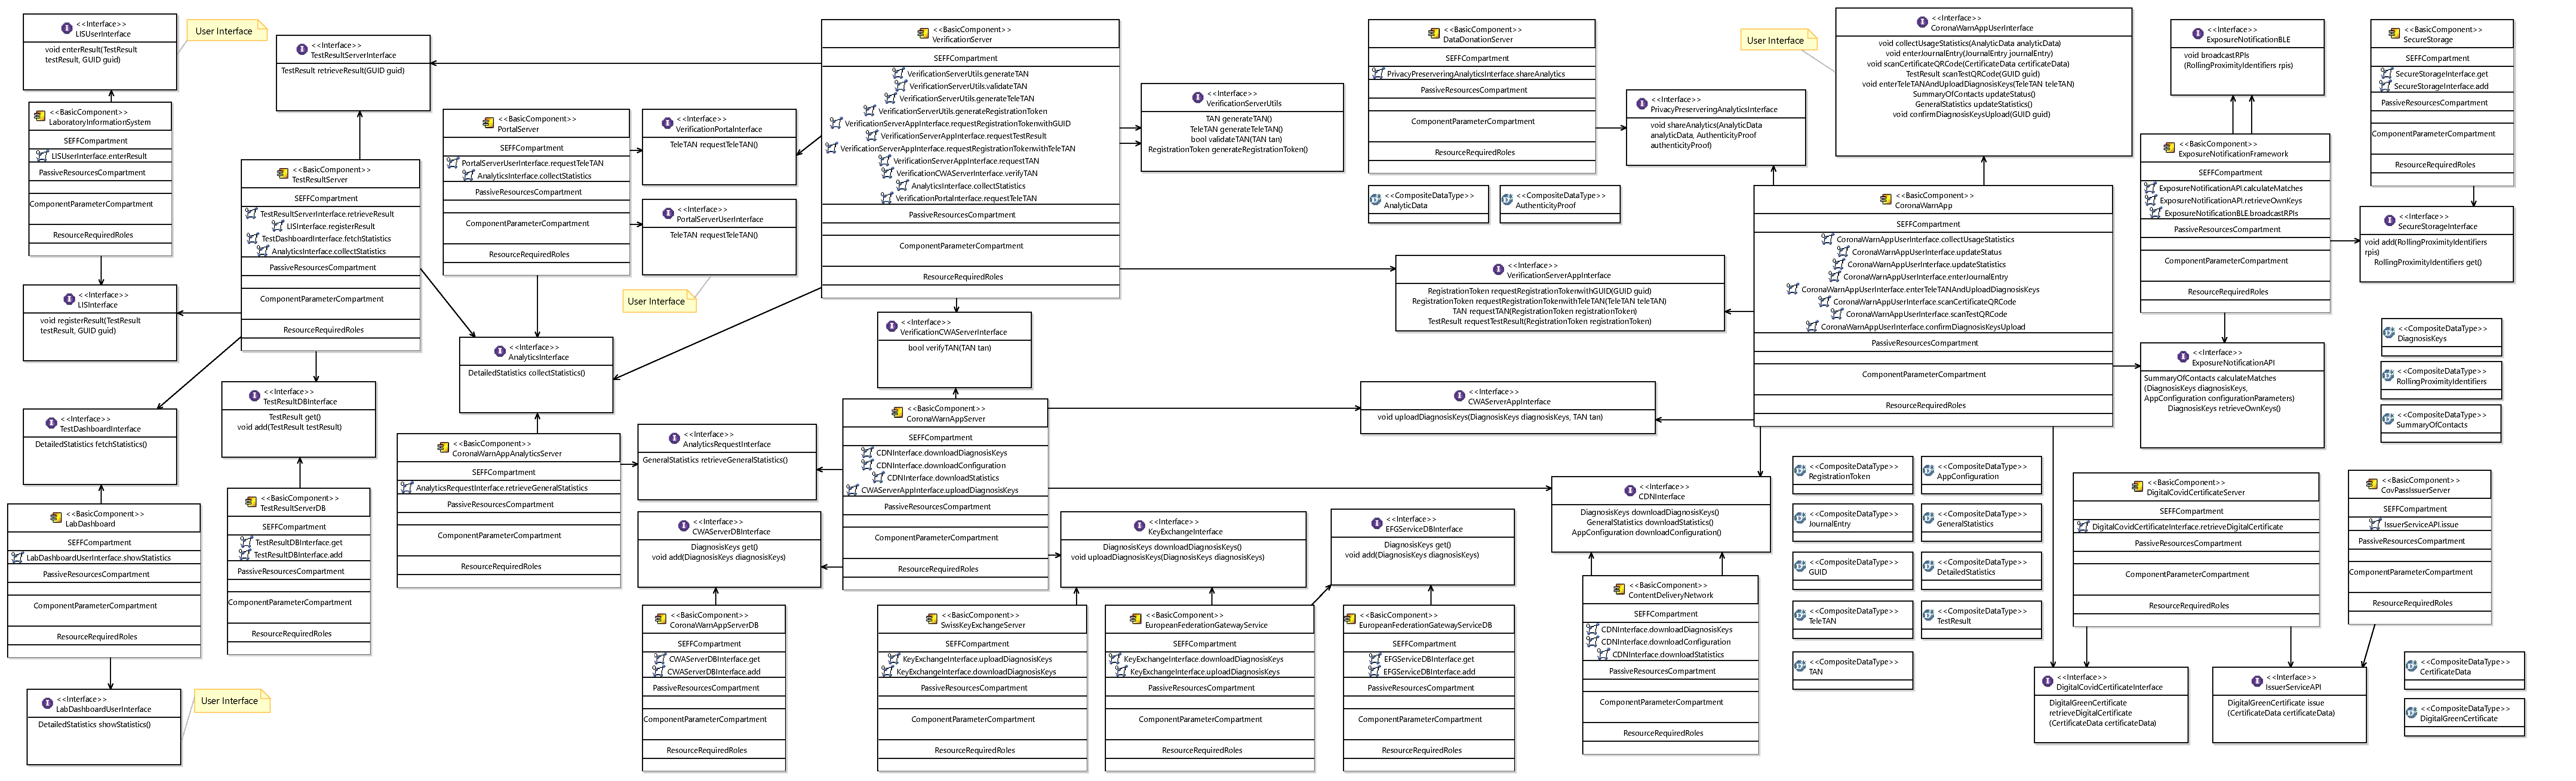
\includegraphics[width=\textwidth]{figures/chapter12/cwa.pdf}
    \caption[Palladio component repository model of the Corona Warn App evaluation scenario (overview).]{Palladio component repository model of the Corona Warn App evaluation scenario (overview), exported from the Palladio-Bench \cite{reussner_palladio_2024}.}
    \label{fig:appendix:cwa:overview}
\end{figure}

\begin{figure}
    \centering
    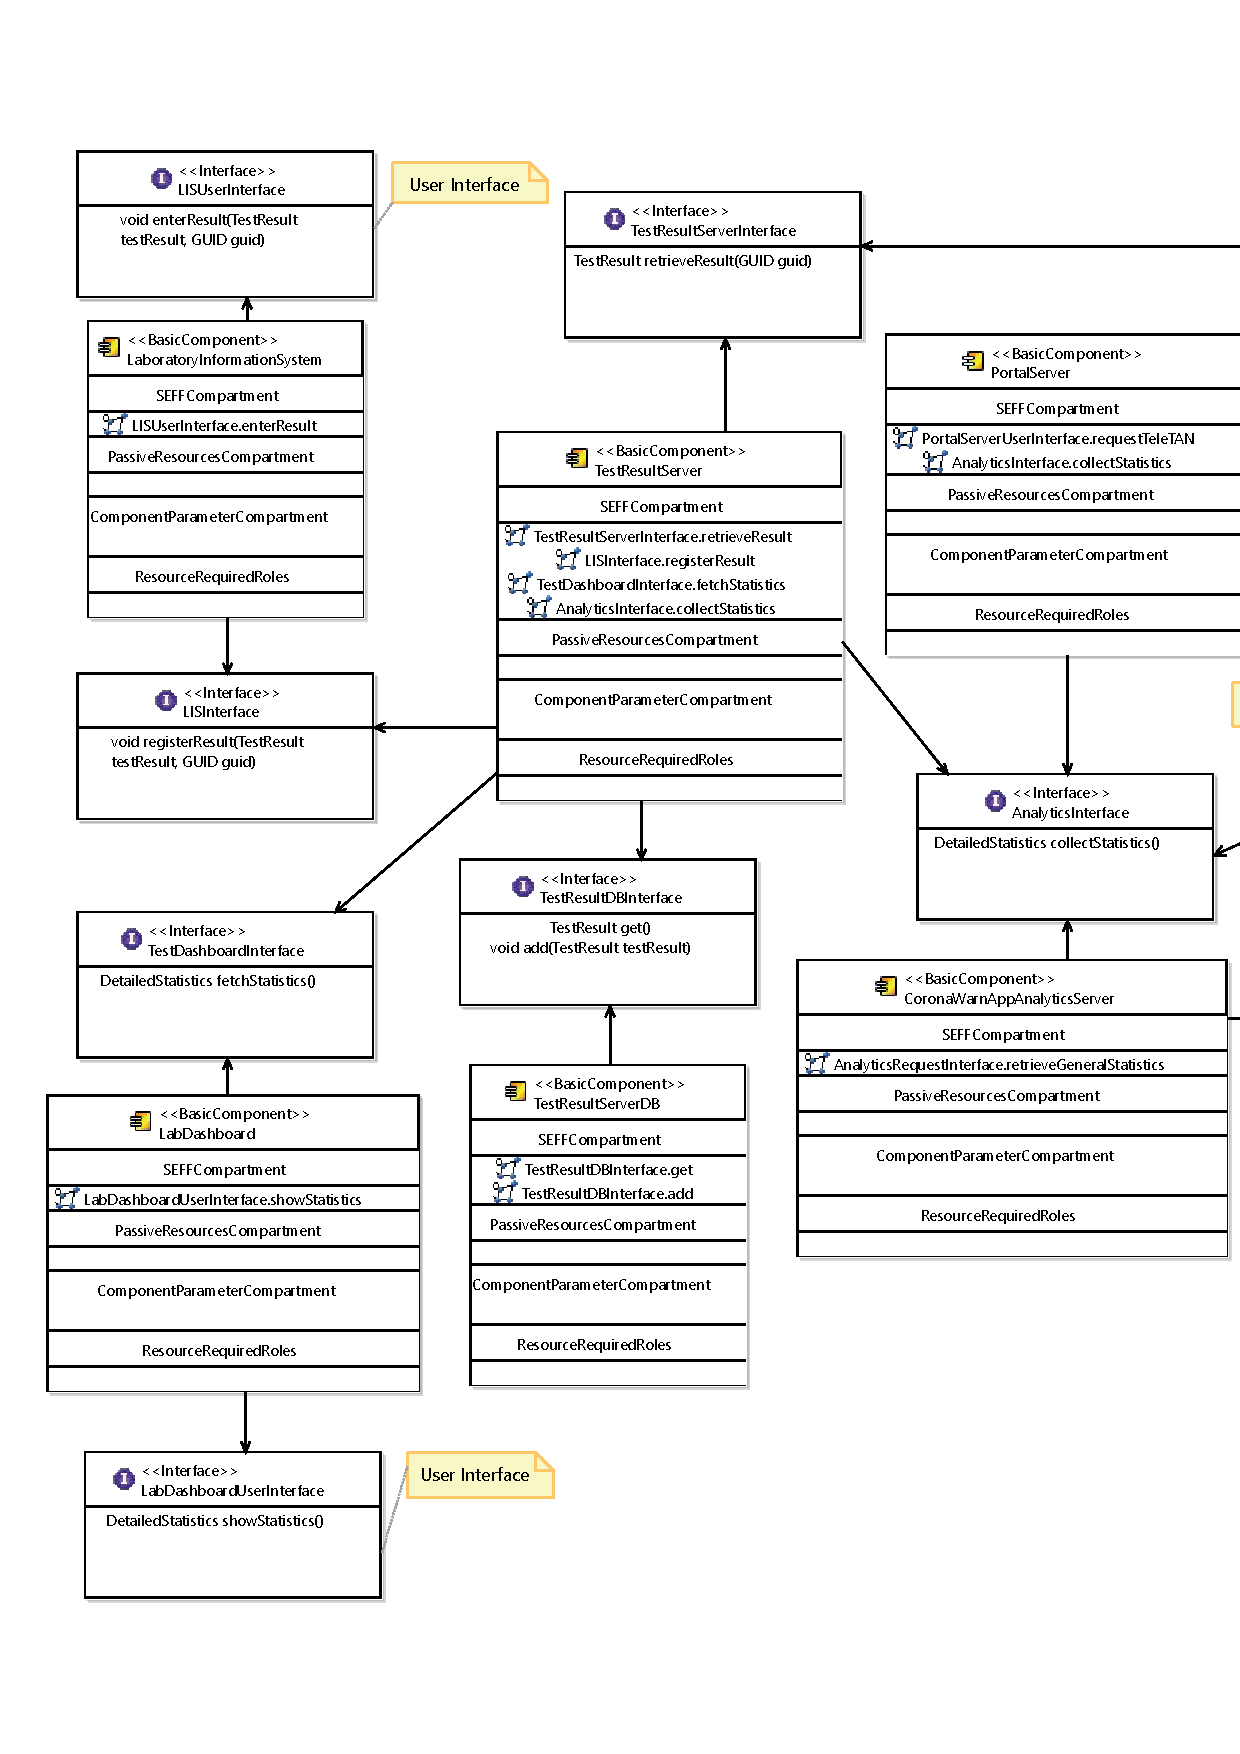
\includegraphics[width=\textwidth]{figures/chapter12/cwa1.pdf}
    \caption[Palladio component repository model of the Corona Warn App evaluation scenario (part 1 of 4).]{Palladio component repository model of the Corona Warn App evaluation scenario (part 1 of 4), exported from the Palladio-Bench \cite{reussner_palladio_2024}.}
    \label{fig:appendix:cwa:1}
\end{figure}

\begin{figure}
    \centering
    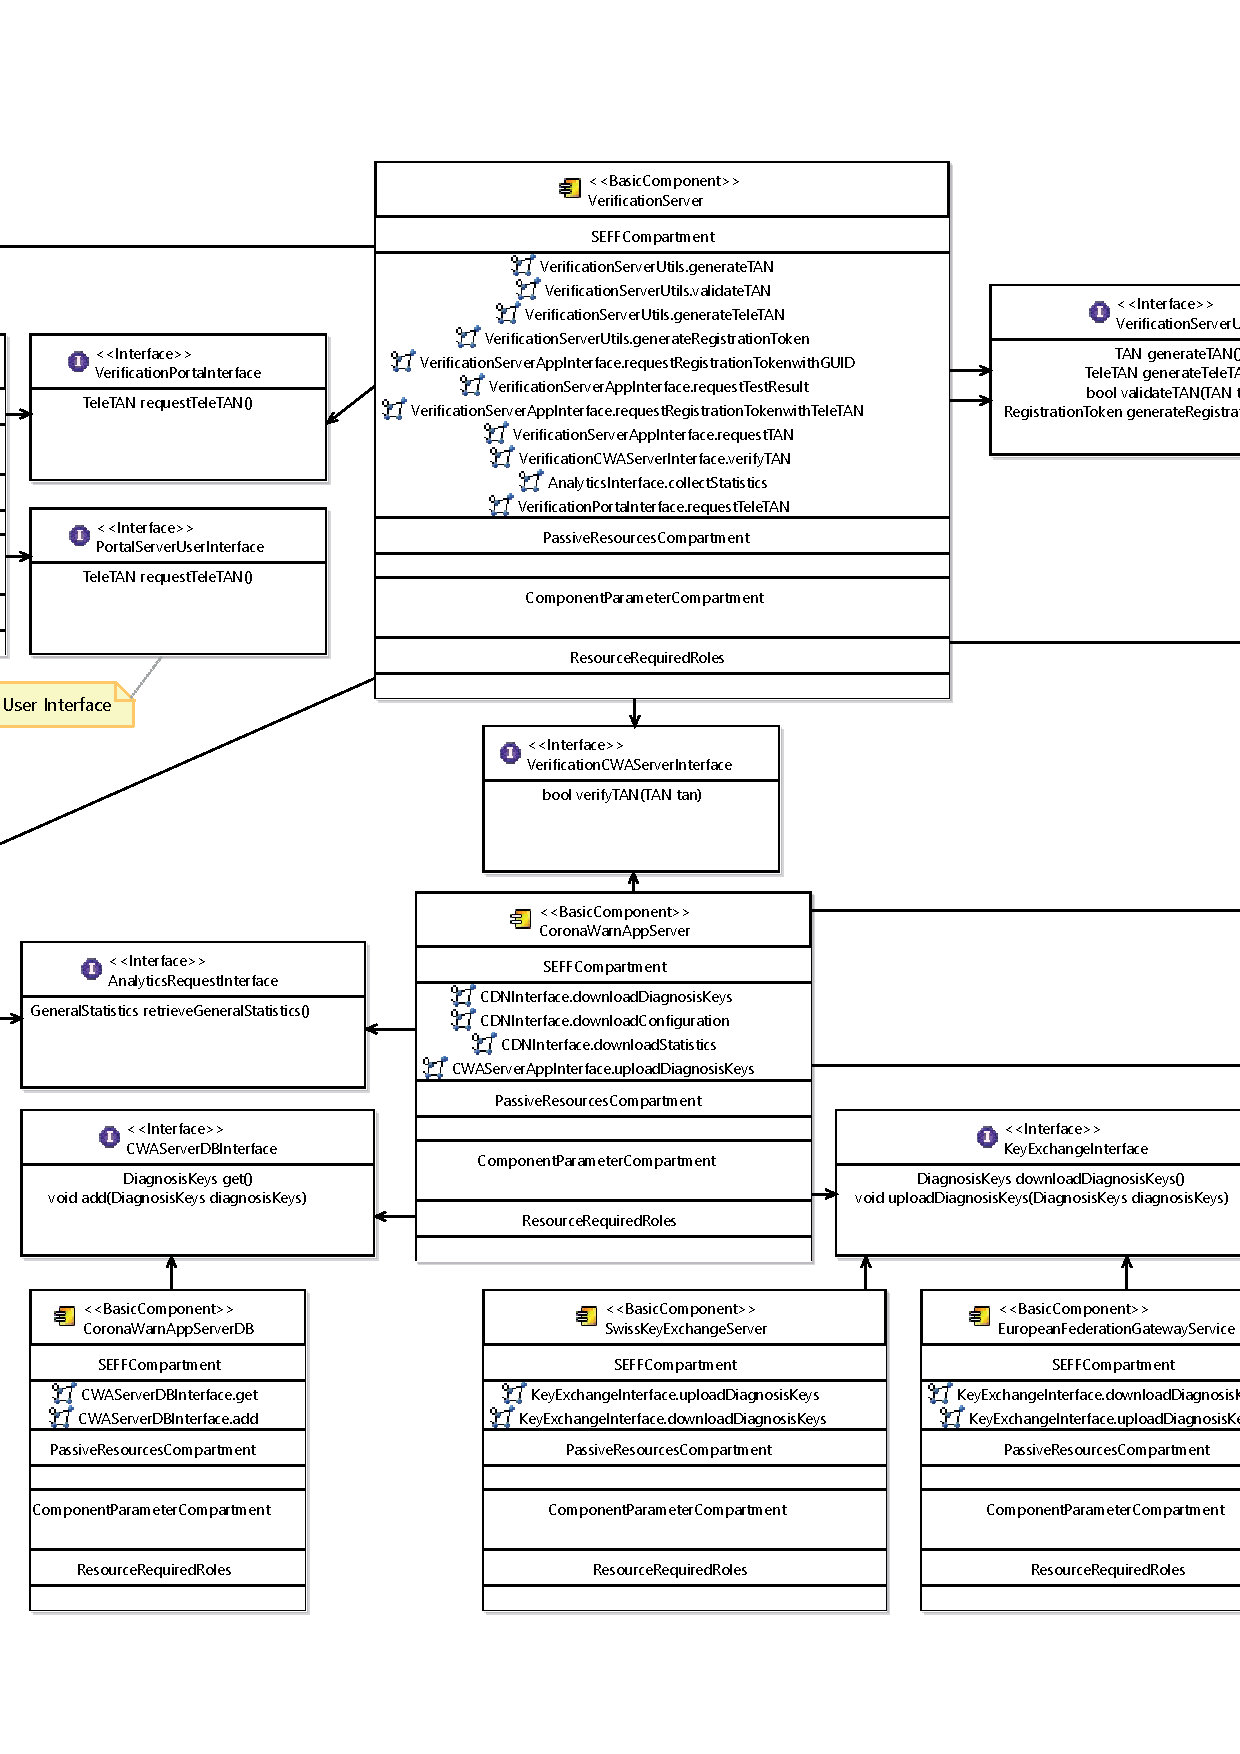
\includegraphics[width=\textwidth]{figures/chapter12/cwa2.pdf}
    \caption[Palladio component repository model of the Corona Warn App evaluation scenario (part 2 of 4).]{Palladio component repository model of the Corona Warn App evaluation scenario (part 2 of 4), exported from the Palladio-Bench \cite{reussner_palladio_2024}.}
    \label{fig:appendix:cwa:2}
\end{figure}

\begin{figure}
    \centering
    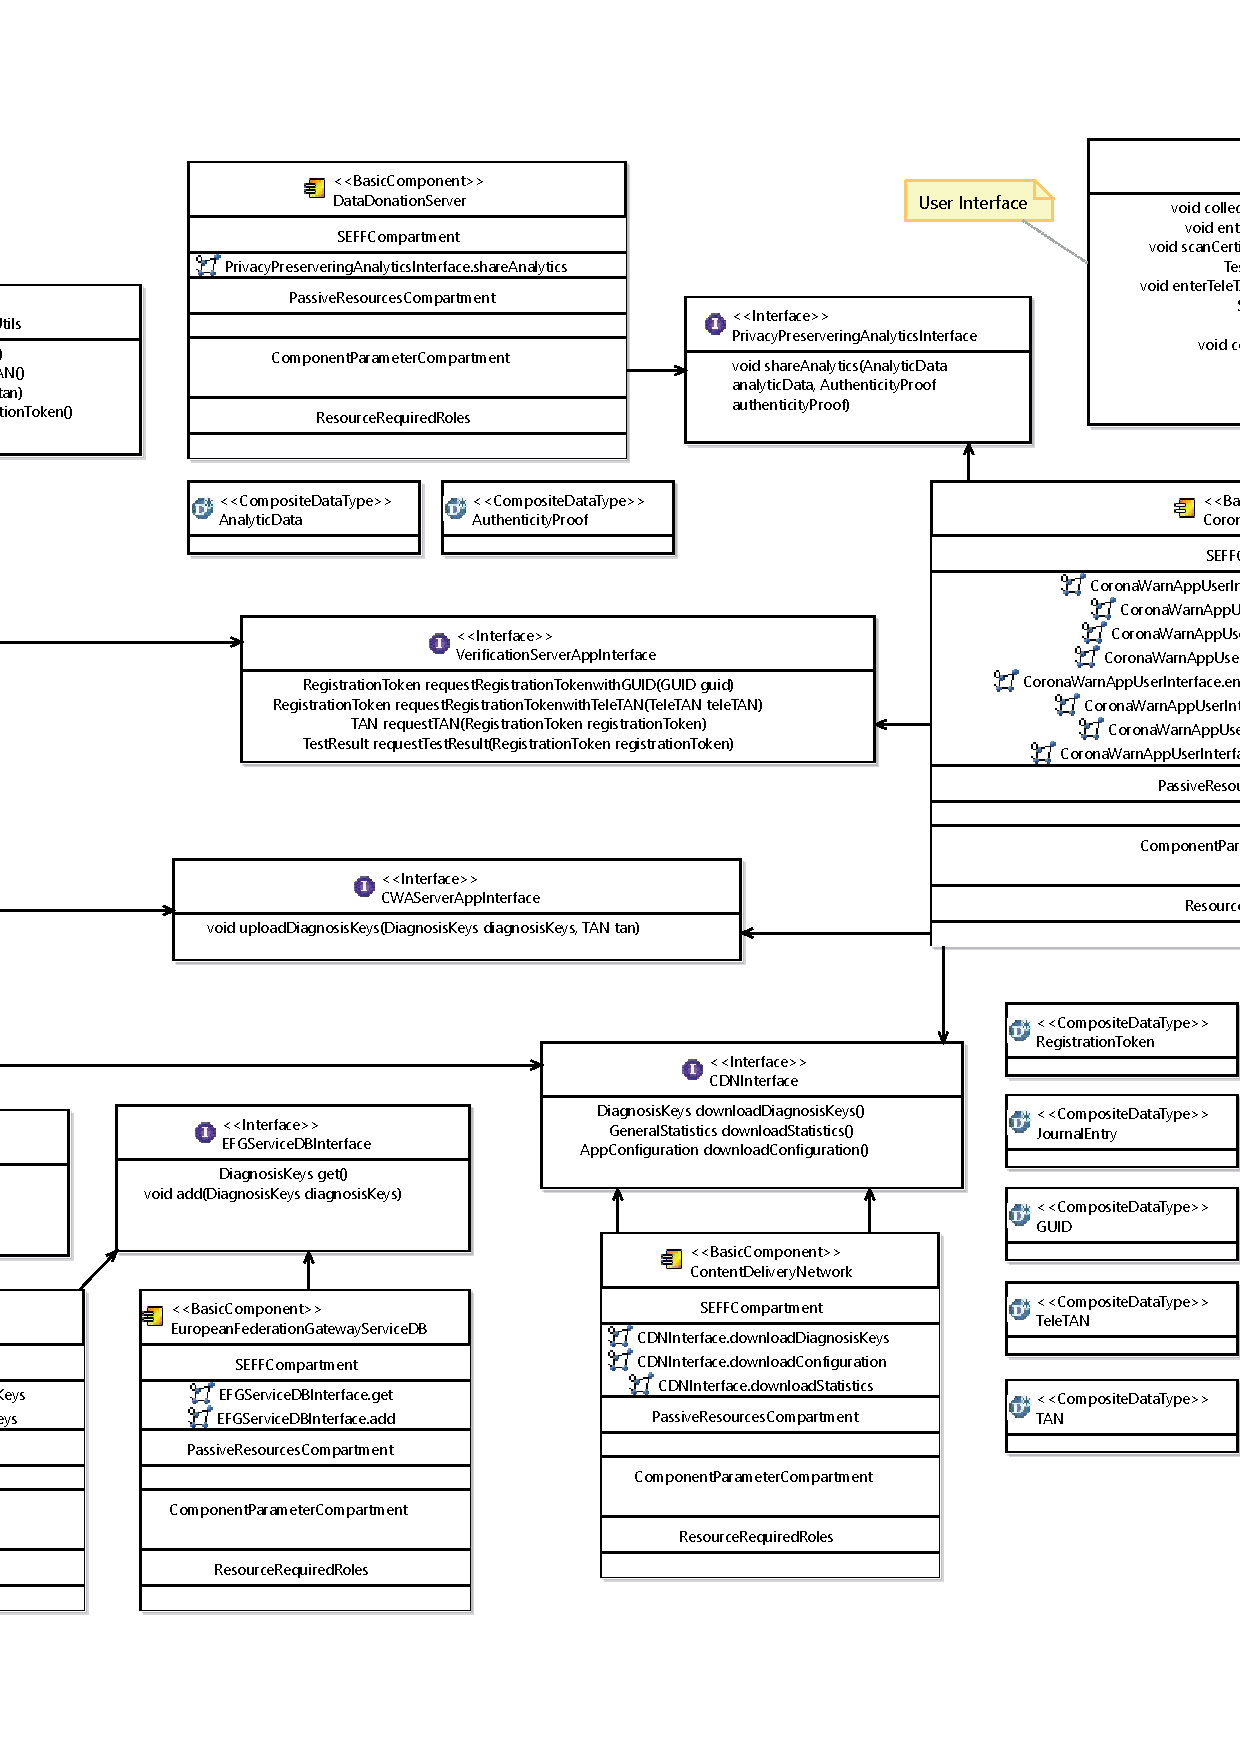
\includegraphics[width=\textwidth]{figures/chapter12/cwa3.pdf}
    \caption[Palladio component repository model of the Corona Warn App evaluation scenario (part 3 of 4).]{Palladio component repository model of the Corona Warn App evaluation scenario (part 3 of 4), exported from the Palladio-Bench \cite{reussner_palladio_2024}.}
    \label{fig:appendix:cwa:3}
\end{figure}

\begin{figure}
    \centering
    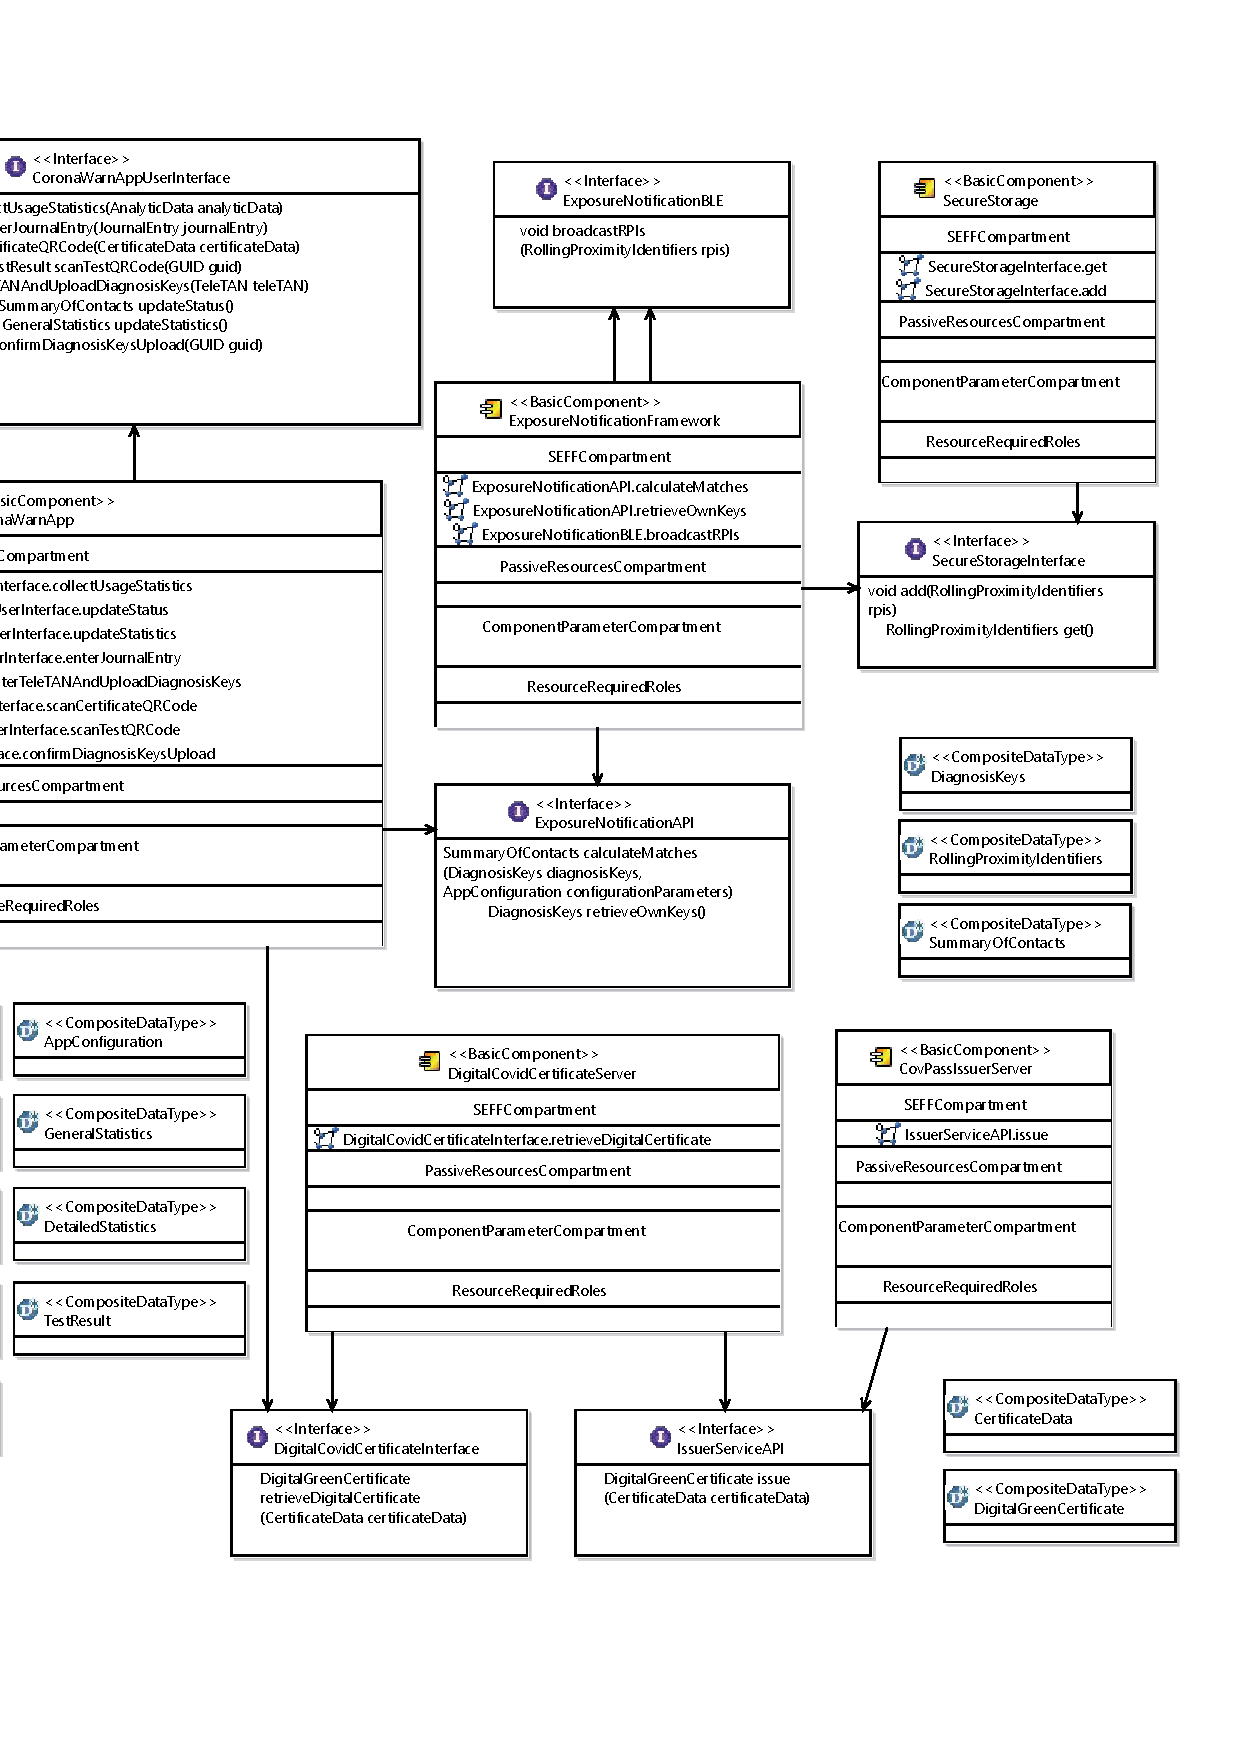
\includegraphics[width=\textwidth]{figures/chapter12/cwa4.pdf}
    \caption[Palladio component repository model of the Corona Warn App evaluation scenario (part 4 of 4).]{Palladio component repository model of the Corona Warn App evaluation scenario (part 4 of 4), exported from the Palladio-Bench \cite{reussner_palladio_2024}.}
    \label{fig:appendix:cwa:4}
\end{figure}





\chapter{Towards a Graphical Notation for Uncertainty in Data Flow Diagrams}%
\label{sec:appendix:ndfd}

As addressed previously in this dissertation, there is an ongoing discussion on standardizing the representation of uncertainty in software models.
\textcite{troya_uncertainty_2021} conducted a \acf{SLR} on the wide variety of existing proposals on the representation of uncertainty and find that it is a \enquote{good time for the modeling community to try to organize their efforts} \cite{troya_uncertainty_2021}.
This includes a consensus on the types of uncertainty, but also appropriate notations.
In this dissertation, we presented five types of uncertainty sources that are relevant regarding confidentiality and we argued why there should not be less or more than these five types, see \autoref{ch:classification}.
Furthermore, we proposed notations for uncertainty in \acfp{DFD} and \acfp{DAG}, see \autoref{sec:classification:dfd} and \autoref{sec:confidentialityanalysis:abunai}.
However, we did intentionally not define a precise graphical notation, as such an endeavor requires a larger consensus like the ongoing effort to define the \acf{PSUM} standard \cite{PSUM}.
Nevertheless, we want to propose an initial graphical notation for uncertainty in \acp{DFD} that might help the ongoing discussion.

\begin{figure}
    \centering
    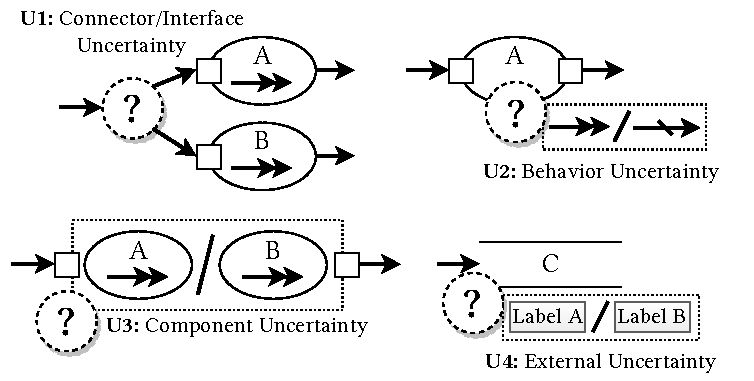
\includegraphics[width=0.9\textwidth]{figures/chapter12/graphicalndfd.pdf}
    \caption{Initial proposal for graphically representing uncertainty in \acfp*{DFD}.}
    \label{fig:appendix:ndfd}
\end{figure}

\autoref{fig:appendix:ndfd} shows our proposal.
Regarding the abstract syntax, we use the elements of our meta model for \acfp{NDFD}, see \autoref{fig:confidentialityanalysis:ndfd}.
The graphical representation of \acp{DFD} follows the concrete syntax of the unified modeling primitives by \textcite{seifermann_unified_2021}.
As specified by \textcite{demarco_structure_1979}, nodes are denoted by circles or lines, depending on their type, and flows are denoted by arrows.
In our example, \emph{A} and \emph{B} represent processes and \emph{C} represents a file.
Pins are denoted by rectangles that decouple flows and nodes, and the behavior specified by assignments is annotated to the nodes.
In our example, we show two different behaviors, denoted with different arrow types, e.g., the two-headed arrow $\twoheadrightarrow$.
Last, node labels are also annotated, e.g., \emph{Label A}, and \emph{Label B}.
For an introduction, see \autoref{sec:foundations:dfd}.

Our \ac{NDFD} meta model shows the relation of the five uncertainty types to the \ac{DFD} element types.
\emph{Connector} and \emph{Interface} uncertainty are \emph{secondary} uncertainty types, that affect the flow between nodes, see \autoref{sec:classification:dfd}.
We denote this using the question mark syntax introduced in \autoref{ch:runningexample}, by annotating the question mark to the alternative flow.
In \autoref{fig:appendix:ndfd}, this is shown as an alternative flow to either node \emph{A} or node \emph{B} due to Uncertainty \U{1}.
\emph{Behavior} uncertainty is \emph{primary} uncertainty, directly affecting a node.
We denote this using the question mark and by showing alternative arrows that represent the behavior.
For instance, the behavior of node \emph{A} could be the forwarding or the encryption of data due to Uncertainty \U{2}.
\emph{Component} uncertainty affects a complete node and thus subsumes \emph{Behavior} and \emph{External} uncertainty.
We denote this again using the question mark syntax and show the alternative nodes, e.g., node \emph{A} and node \emph{B} due to Uncertainty \U{3}.
A benefit of this graphical notation is that it shows that both nodes require the same interface, i.e., the same pins.
Last, \emph{External} uncertainty affects node labels.
We denote this using the question mark and by enumerating alternative labels, see Uncertainty \U{4}.

Although this graphical notation has many benefits, e.g., directly representing the different scenarios, it is not perfect yet.
For instance, we cannot represent the difference between \emph{Connector} and \emph{Interface} uncertainty.
Additionally, we cannot represent the impact of \emph{Connector} uncertainty on the assignments of the outgoing node.
Last, to avoid ambiguity, we always have to specify the variation due to the uncertainty, e.g., the different labels, or different behaviors.
Otherwise, the graphical syntax would, e.g., not differentiate between \emph{Behavior} and \emph{External} uncertainty.
Due to these shortcomings, we felt not confident to claim this graphical syntax as part of our contributions.
Instead, we focused on the representation of uncertainty in \acp{DAG} that is more straightforward by only differentiating between \emph{primary} and \emph{secondary} uncertainty.
However, in the light of the recent standardization efforts \cite{PSUM} and to address the need for discussing uncertainty in \acp{DFD} based on drawing diagrams, we conclude this dissertation with this short proposal\footnote{%
\textbf{Acknowledgement}: Not a single sentence of this dissertation was generated by ChatGPT, Gemini, LLaMA, or a comparable tool.
We only used the language-related tools DeepL (\href{https://www.deepl.com/}{https://www.deepl.com/}) and Grammarly (\href{https://grammarly.com/}{https://grammarly.com/}) to correct spelling and grammatical mistakes.}.
